\section{Qualia as Boundary Phenomenon}


本節では、クオリアを本稿の構造の中に位置づける。

ここで行うのは、クオリアを否定することではない。

また、クオリアを意識の中心に置くことでもない。

本稿の立場では、クオリアは意識そのものではない。

それは、ログ参照が開かれつつある境界で現れる、現象的な前景である。

\subsection{Why the Qualia Problem Does Not Converge}

クオリア問題は、長いあいだ意識研究の中心に置かれてきた。

赤の赤さ。

痛みの痛さ。

音の響き。

今ここにある感じ。

これらは、確かに経験される。

そのため、クオリアを否定することはできない。

しかし、クオリアを意識の本体として扱うと、議論は収束しにくくなる。

理由は単純である。

クオリアは、保存された対象ではないからである。

クオリアを「どこにあるのか」「何として保存されているのか」「どの表象に対応するのか」と問うと、問いは最初からずれる。

それは、流れている境界を、固定された物体として探すことに近い。

本稿では、クオリア問題が終わらない理由を、神秘性ではなく、位置づけの誤りとして捉える。

クオリアは、内部に存在する何かではない。

それは、処理がログとして沈殿しつつある境界で、一時的に現れる現象である。

\subsection{Qualia as Sedimentation Frontier}

本稿では、クオリアを沈殿前線として位置づける。

高速層では、予測、反応、誤差、行動候補が揮発的に走る。

低速層では、それらの一部がログとして沈殿し、再参照可能な構造になる。

クオリアは、この二つの層のどちらか一方に属するものではない。

それは、高速層の処理が低速層へ沈殿しようとする境界に現れる。

この境界を、沈殿前線、または closure frontier と呼ぶことができる。

ここでいう closure は、完全閉包を意味しない。

処理が完全に閉じてしまえば、それはすでにログ、記憶、ラベル、概念になっている。

一方で、まったく閉じなければ、処理は痕跡を残さず流れ去る。

クオリアは、その中間にある。

閉じようとしているが、まだ閉じ切っていない。

流れているが、すでに沈殿へ向かっている。

この過渡状態が、クオリアとして経験される。

\cref{fig:qualia-boundary-ja} は、クオリアを一時的な境界状態として位置づける。

\begin{figure}[H]
\centering
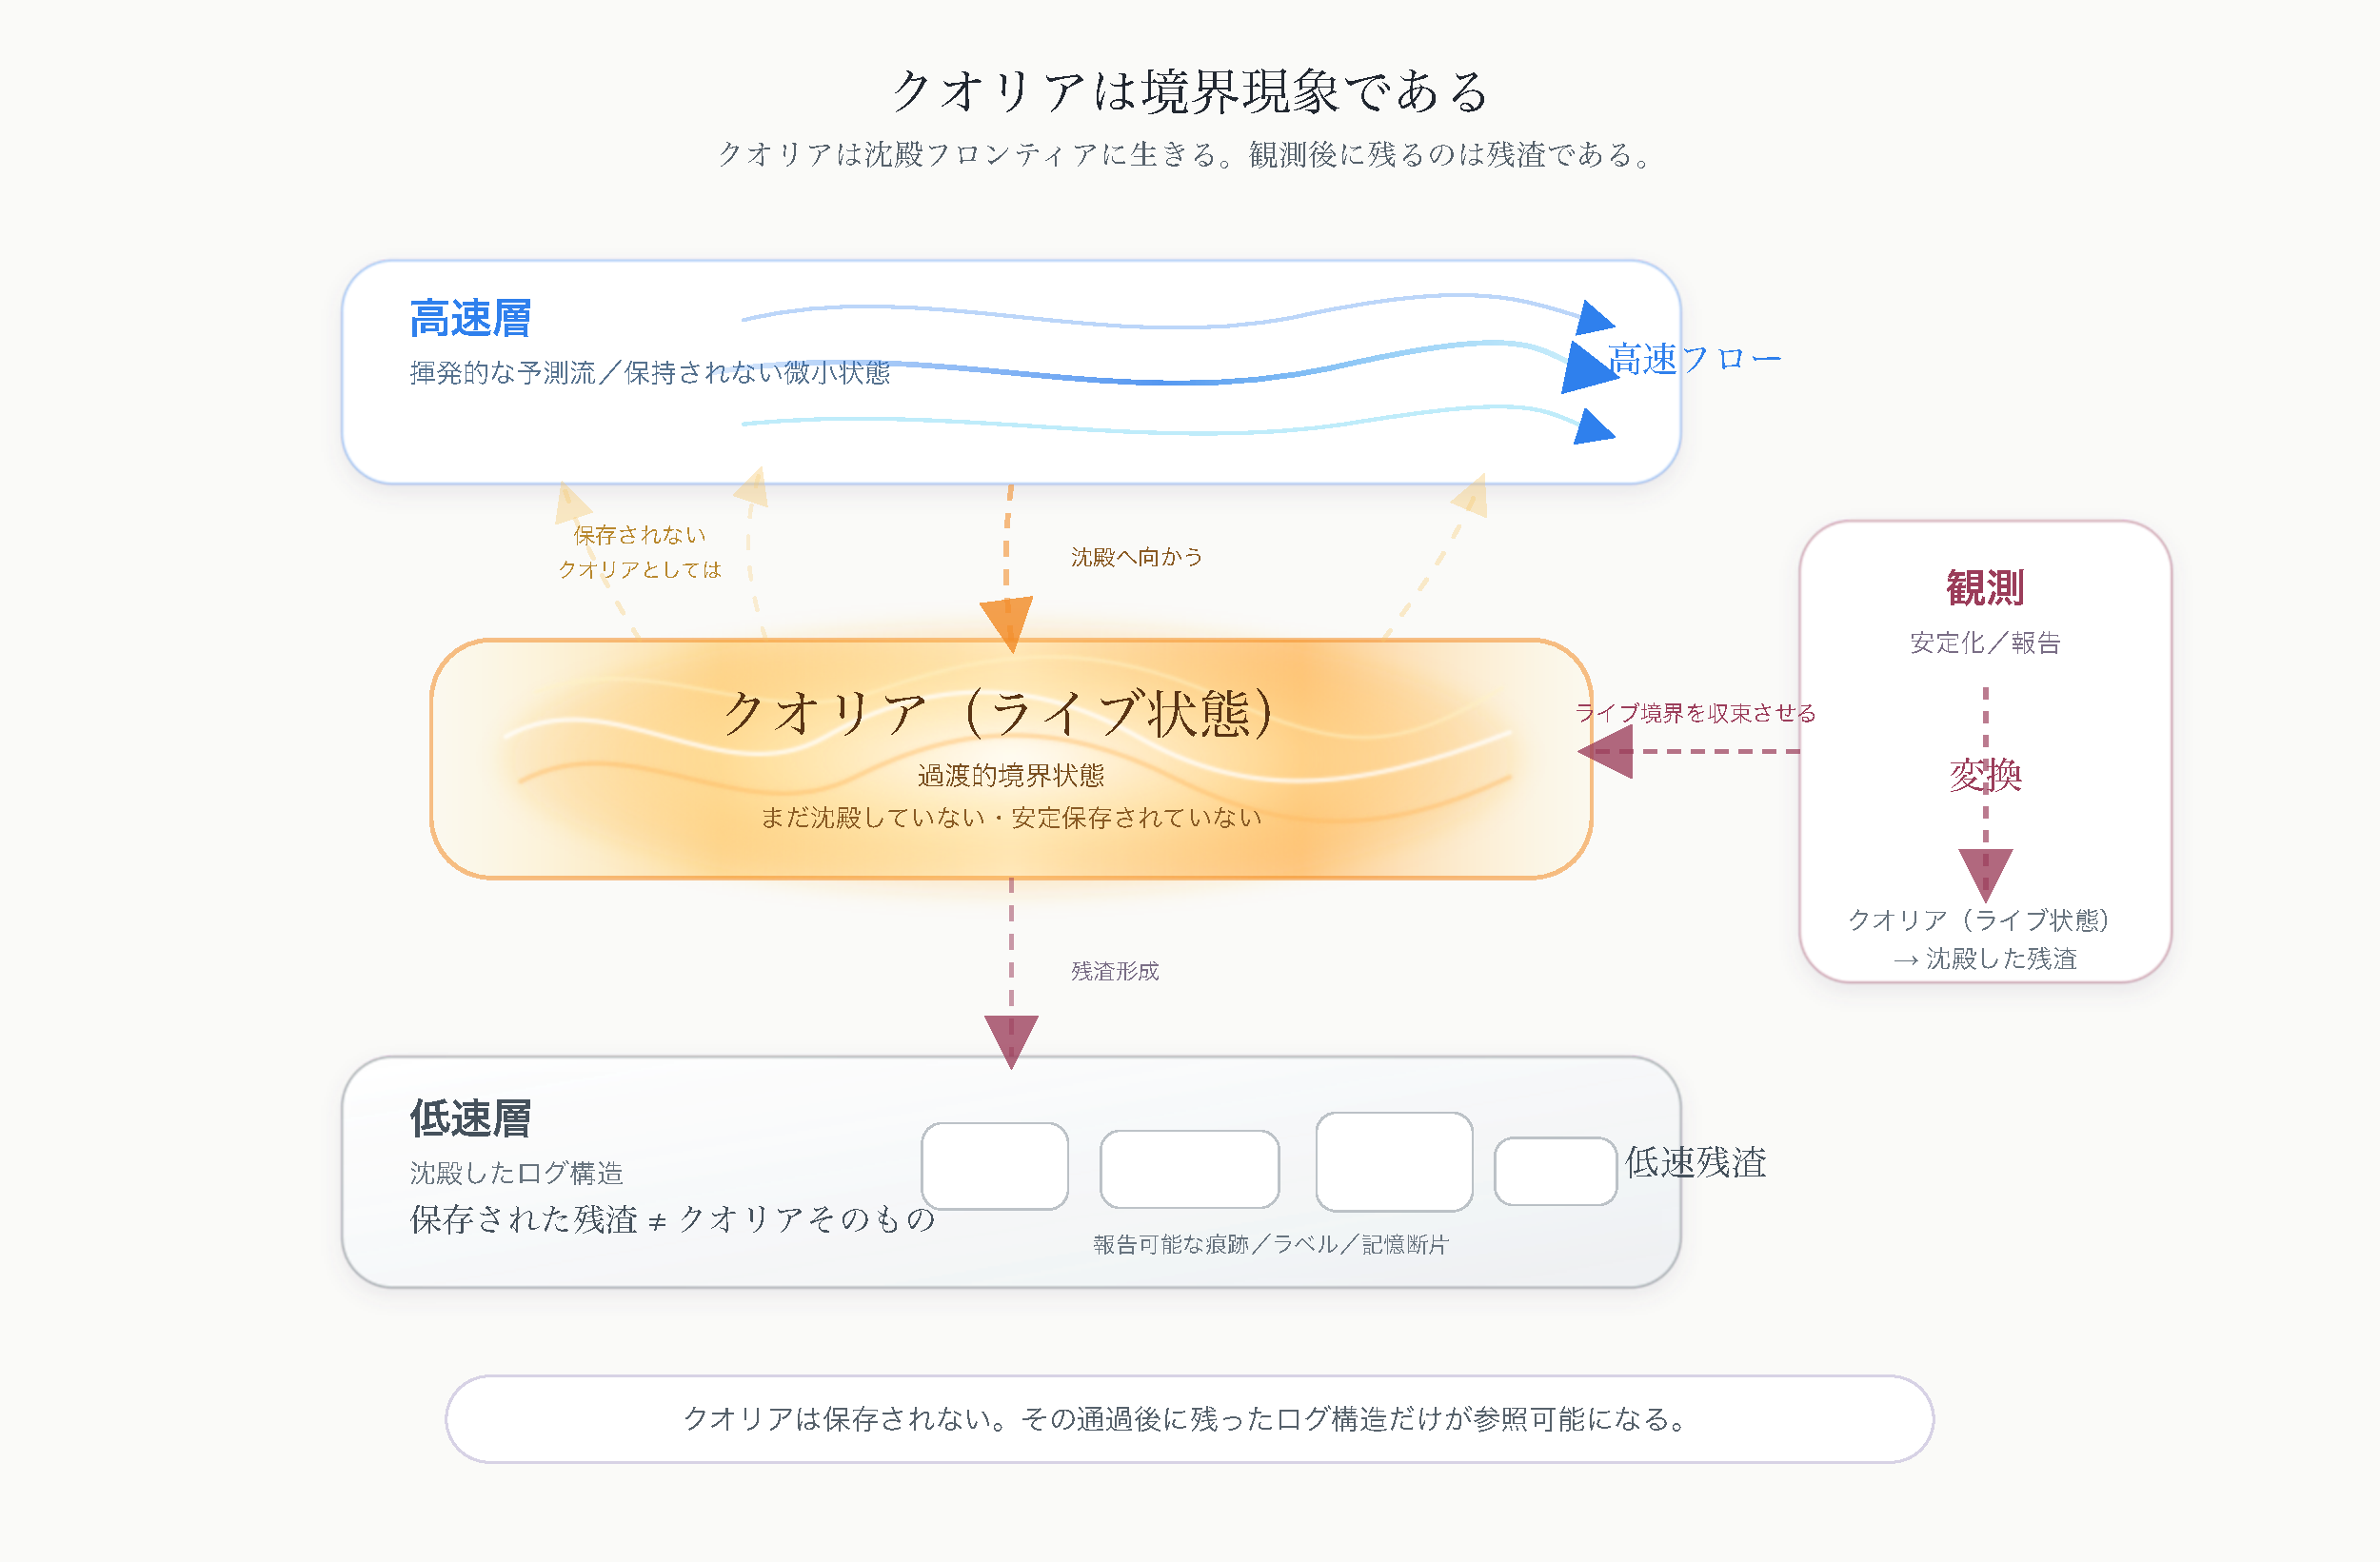
\includegraphics[width=0.92\linewidth]{figures_ja/figure5_qualia_boundary_jp.pdf}
\caption{
境界現象としてのクオリア。
クオリアは、高速な予測流と低速なログ構造のあいだの沈殿前線にライブに現れる。
測定はこのライブな境界を安定化し、沈殿残余へ変換する。
再参照可能なものとして残るのはクオリアそのものではなく、その通過後に残されたログ構造である。
}
\label{fig:qualia-boundary-ja}
\end{figure}

\subsection{Qualia Are Live, Not Stored}

クオリアは保存されない。

この言い方は強く見えるかもしれない。

しかし、ここで意味しているのは、クオリアが存在しないということではない。

クオリアは存在する。

ただし、それは保存物として存在するのではなく、ライブな境界状態として存在する。

たとえば、痛みの記憶は残る。

赤を見たという記憶も残る。

音楽を聴いたという記憶も残る。

しかし、残っているのはクオリアそのものではない。

残っているのは、クオリアが通過した後のログ構造である。

記憶として再生されるものは、かつてのクオリアではなく、クオリアを伴って更新された低速層の痕跡である。

したがって、クオリアを忠実に保存しようとする試みは、構造的に失敗する。

保存された瞬間、それはすでにクオリアではなく、ログになっている。

\subsection{Qualia and the Plasticity Gate}

クオリアは、可塑性ゲートの近傍で現れる。

高速層の処理が低速層へ沈殿するためには、可塑性ゲートを通過しなければならない。

このゲートが完全に閉じていれば、処理は経験として残らない。

このゲートが完全に開きすぎていれば、処理は過剰に沈殿し、固定化しやすくなる。

クオリアは、そのゲートが開きつつあり、しかしまだ沈殿が完了していない状態に現れる。

したがって、クオリアはゲートの産物ではない。

それは、ゲートを通過しつつある処理の現象的側面である。

この意味で、クオリアはログ参照の結果でもあり、ログ沈殿の途中経過でもある。

完全に高速層側にあれば、まだ報告可能ではない。

完全に低速層側に入れば、すでに記憶や言語ラベルになっている。

クオリアは、その境界でだけライブに現れる。

\subsection{Qualia and Effective Torque}

クオリアの明瞭さは、単なる刺激の強度だけでは決まらない。

本稿の枠組みでは、クオリアは速度差、結合粘性、意味勾配の組み合わせによって変化する。

この関係は、有効トルク様量として次のように表される。

\begin{equation}
\mathcal{T}_{\Phi}
\sim
\kappa
\frac{\Delta v}{\mu}
|\nabla \Phi|
\end{equation}

$\mathcal{T}_{\Phi}$ が小さすぎる場合、処理は十分な参照方向を持たず、クオリアはぼんやりする。

$\mathcal{T}_{\Phi}$ が中間領域にある場合、処理は低速層へ沈殿しつつも、まだライブな境界として保たれる。

このとき、クオリアは明瞭でありながら、固定されすぎない。

一方で、$\mathcal{T}_{\Phi}$ が大きすぎる場合、処理は特定の意味井戸へ過剰に引き込まれる。

この場合、クオリアは強く感じられるかもしれない。

しかし、その強さは必ずしも自由な意識状態を意味しない。

むしろ、意味勾配が強すぎることで、クオリアが特定の記憶や物語へ固定されやすくなる。

したがって、クオリアの明瞭さと意識の安定性は同義ではない。

\subsection{Measurement Converts Qualia into Residue}

クオリアは測定によって変質する。

これは、クオリアが神秘的だからではない。

クオリアが境界現象だからである。

測定とは、対象を安定化し、報告可能にし、比較可能にする操作である。

しかし、クオリアは安定化される前の境界にある。

そのため、測定しようとすると、クオリアは低速層へ沈殿し、ログ、ラベル、報告、数値、神経的要約へと変換される。

測定後に残るものは、クオリアそのものではない。

それは、クオリアが通過した後の残余である。

この関係は次のように表せる。

\begin{equation}
\text{qualia live}
\rightarrow
\text{measurement}
\rightarrow
\text{sedimented residue}
\end{equation}

したがって、クオリアが測れないという主張は、「何も観測できない」という意味ではない。

観測できるのは、クオリアそのものではなく、クオリアが沈殿した後の痕跡である。

\subsection{Why Qualia Feel Central}

クオリアは意識の本体ではない。

しかし、体験上は非常に中心的に感じられる。

この理由は、クオリアがログ参照のライブな境界に現れるからである。

人間が「いま意識している」と感じる瞬間には、何らかの処理が沈殿しつつあり、同時にまだ完全にはログ化されていない。

その境界で、感覚は鮮明に現れる。

そのため、クオリアは原因であるかのように見える。

しかし、構造的には、クオリアは原因ではない。

それは、処理と沈殿の境界で観測される前景である。

光が物体の存在そのものではなく、物体と観測条件の関係として現れるように、クオリアもまた、処理とログ沈殿の関係として現れる。

このため、クオリアを中心に置くと意識は神秘化される。

しかし、クオリアを境界に置くと、意識はログ参照構造として読み直せる。

\subsection{Relation to the Hard Problem}

いわゆる hard problem は、クオリアを固定された説明対象として扱うところから生じる。

なぜこの神経活動が「この感じ」を伴うのか。

なぜ物理過程が主観的経験になるのか。

この問いは強力である。

しかし、本稿の立場では、この問いはクオリアを保存物として扱っている。

本稿では、クオリアを保存物ではなく、沈殿境界のライブな前景として扱う。

この場合、問うべきことは変わる。

「クオリアはどこにあるのか」ではない。

「どのような条件で、処理はログ化される直前の境界として経験されるのか」である。

この問いに対しては、速度差、結合粘性、内部遅延、意味勾配、可塑性ゲートという構造で答えることができる。

したがって、本稿は hard problem を解いたとは言わない。

むしろ、hard problem を、解けない対象問題から、記述可能な境界条件の問題へ移す。

\subsection{Summary}

本節では、クオリアを境界現象として位置づけた。

\begin{itemize}
\item クオリアは意識の本体ではない。
\item クオリアは保存された対象ではない。
\item クオリアは高速層と低速層の沈殿前線に現れる。
\item クオリアは可塑性ゲートの近傍でライブに成立する。
\item 測定はクオリアを残余へ変換する。
\item クオリアの明瞭さは、$\Delta v$、$\mu$、$\tau$、$\nabla \Phi$、$\mathcal{T}_{\Phi}$ に依存する。
\item hard problem は、クオリアを対象として探す限り収束しない。
\end{itemize}

したがって、クオリアとは、ログ参照が沈殿しつつある境界で現れる、非保存的なライブ前景である。

次節では、この境界現象を含めた意識全体を、生成モデルではなく opening model として整理する。
